% Preamble snippets you likely need:
% \usepackage{graphicx}
% \usepackage{siunitx}

\part{Sensoren für IoT}

% ============================================================
% Device 1: CQRobot TDS sensor (ASIN B08KXRHK7H)
% ============================================================
\section[nosectionpage]{Totaly Disolved Solids (TDS) Sensor}
\begin{frame}{TDS Sensor (B08KXRHK7H): What it Measures}
\begin{columns}[T,onlytextwidth]
  \begin{column}{0.62\textwidth}
    \begin{itemize}
\item \textbf{TDS = Total Dissolved Solids} (ppm) \\
            $\rightarrow$ proxy via \textbf{electrical conductivity}
\item Typischer Einsatz: Monitoring der Wasserqualität (Süßwasser / Hydroponik / Labore)
\item Dieses Board liefert \textbf{analoge Spannungsausgänge} für einen Mikrocontroller
\item Versorgungsspannungsbereich: funktioniert mit \textbf{3.3\,V bis 5\,V‑Klasse}‑Versorgungen
\item Practical note: \textbf{temperature compensation} improves accuracy
    \end{itemize}
  \end{column}
  \begin{column}{0.38\textwidth}
    \centering
    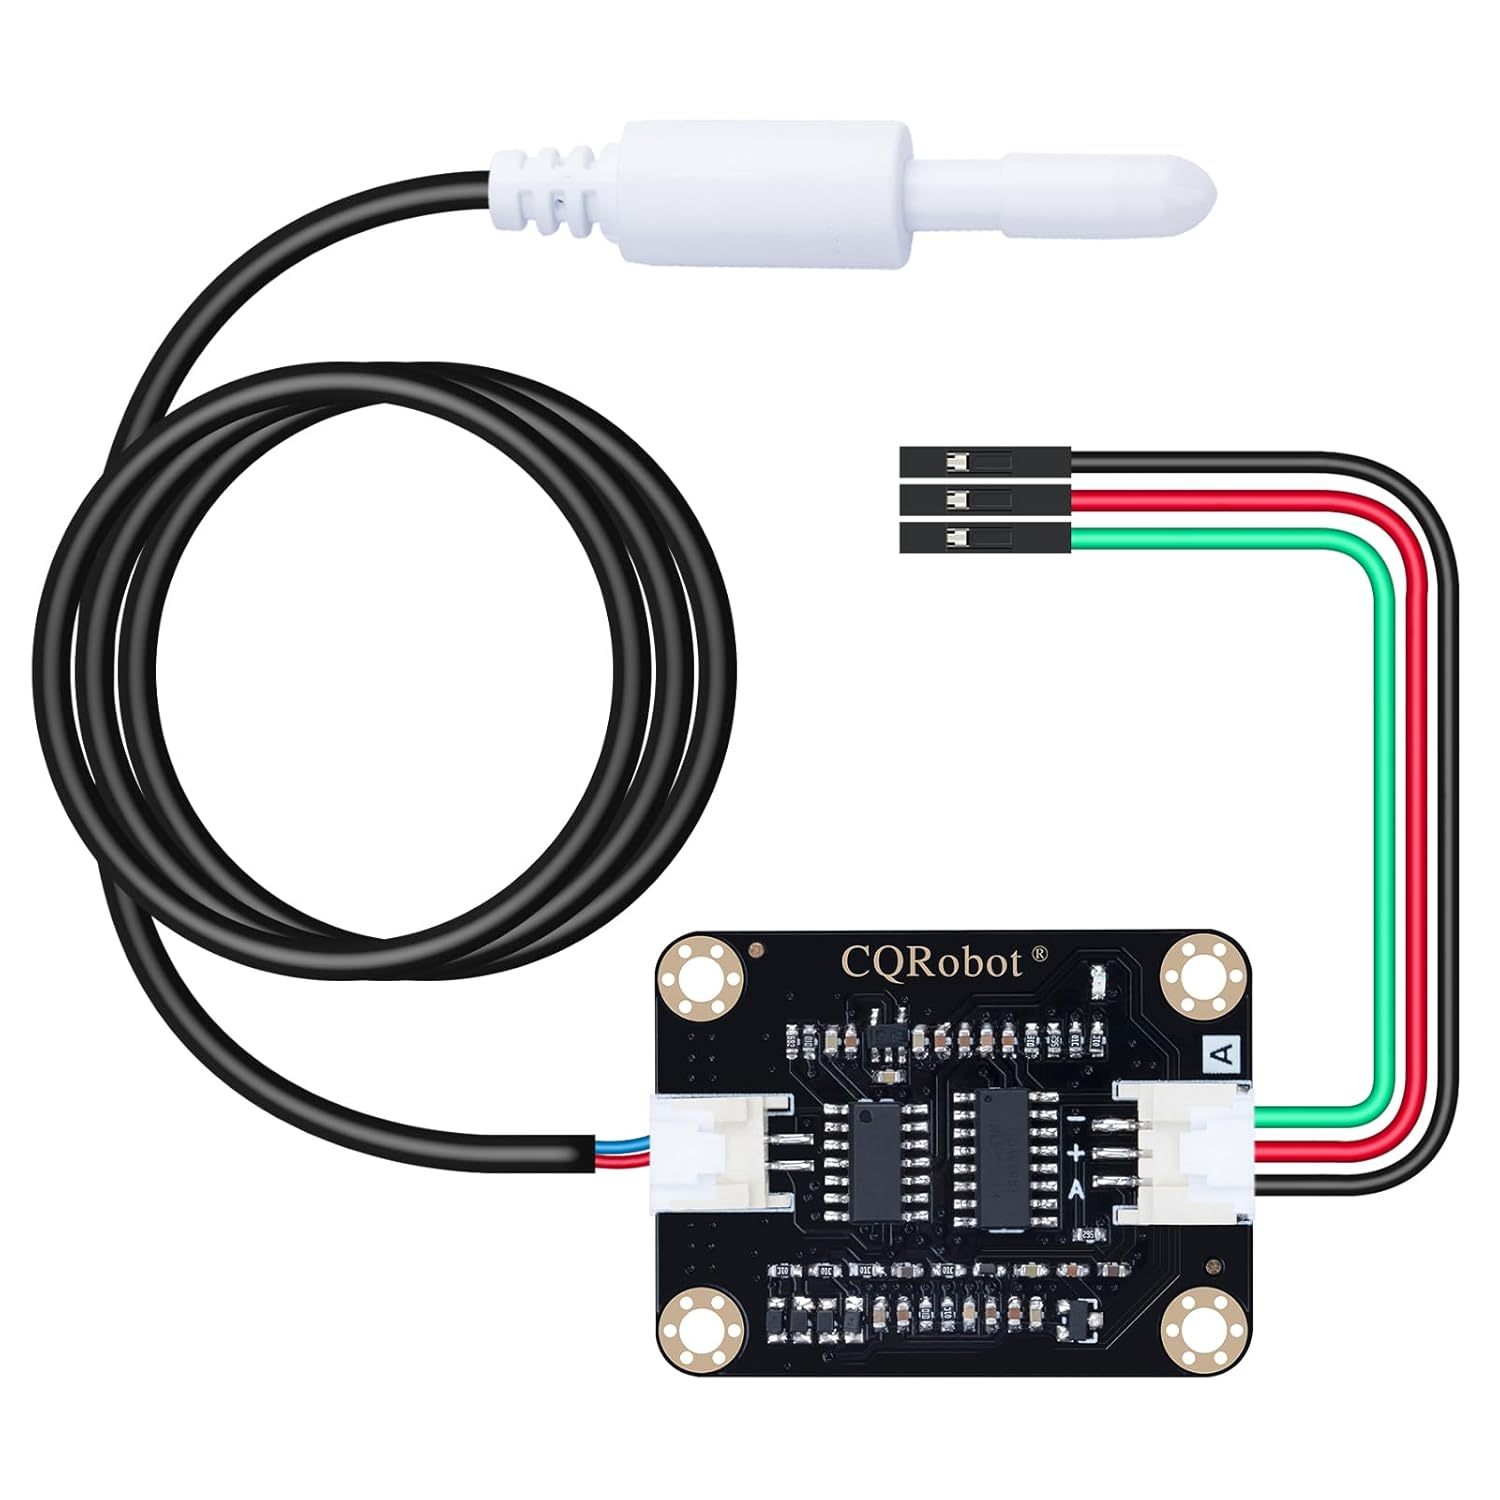
\includegraphics[width=0.8\linewidth]{figures/TDS}\\
    \scriptsize Example: CQRobot TDS module + probe
  \end{column}
\end{columns}
\end{frame}

% \begin{frame}{TDS sensor + ESP32: Wiring \& Usage}
% \begin{columns}[T,onlytextwidth]
%   \begin{column}{0.62\textwidth}
%     \begin{itemize}
% \item \textbf{Versorgung:} an 3.3\,V (oder 5\,V falls erforderlich) + GND anschließen
% \item \textbf{Signal:} analog OUT $\rightarrow$ \textbf{ESP32 ADC1 pin}
% %             \begin{itemize}
% \item Verwenden Sie \textbf{ADC1} (ADC2 kollidiert beim ESP32 mit Wi‑Fi)
% \item Oversample + average (e.g., 50--200 samples)
% %             \end{itemize}
% \item \textbf{Umrechnung:} Spannung \$\rightarrow\$ Leitfähigkeit/TDS mittels Herstellerformel
% \item Optional: \textbf{externen ADC (ADS1115)} für bessere Auflösung verwenden
%     \end{itemize}
%     \vspace{0.3em}
%     \footnotesize
%     Tip: keep the probe clean; avoid bubbles; measure in flowing water for stability.
%   \end{column}
%   \begin{column}{0.38\textwidth}
%     \centering
% %    \includegraphics[width=\linewidth]{figures/tds_wiring_ads1115.png}\\
%     \scriptsize Example wiring with external ADC
%   \end{column}
% \end{columns}
% \end{frame}

% ============================================================
% Device 2: Turbidity sensor module (ASIN B07SLRRX38 / TSW-20M)
% ============================================================
\section[nosectionpage]{Turbidity Sensor}
\begin{frame}{Turbidity Sensor (B07SLRRX38 / TSW-20M): Überblick}
\begin{columns}[T,onlytextwidth]
  \begin{column}{0.62\textwidth}
    \begin{itemize}
\item \textbf{Trübung} = „Trübheit“ durch Partikel im Wasser (optische Methode)
\item Einsatzbereiche: Abwasser, Flüsse/Seen, Monitoring von Wasch-/Geschirrspülvorgängen
\item Module typically provides:
            \begin{itemize}
\item \textbf{Analog output} (continuous turbidity signal)
\item \textbf{Digital output} (threshold comparator)
            \end{itemize}
\item Häufig versorgt über \textbf{5\,V} (Sensor + Conditioning-Board)
    \end{itemize}
  \end{column}
  \begin{column}{0.38\textwidth}
    \centering
    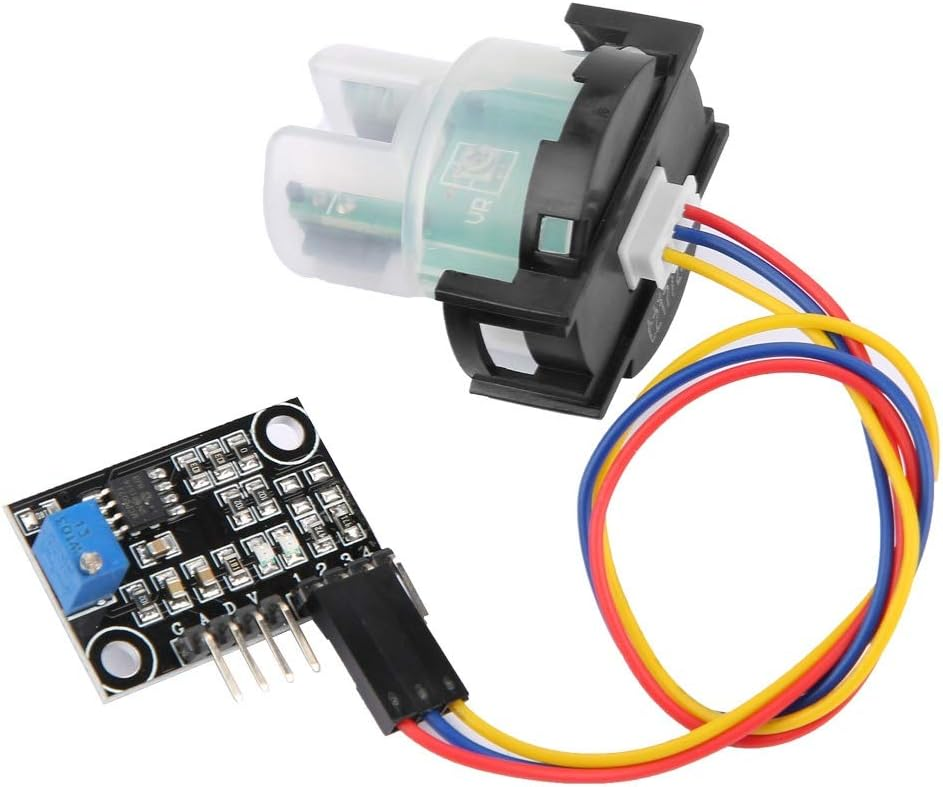
\includegraphics[width=0.8\linewidth]{figures/Turbidity}\\
    \scriptsize TSW-20M style turbidity sensor + board
  \end{column}
\end{columns}
\end{frame}

% \begin{frame}{Turbidity + ESP32: Practical Integration}
% \begin{columns}[T,onlytextwidth]
%   \begin{column}{0.62\textwidth}
%     \begin{itemize}
% \item \textbf{Versorgung:} 5\,V + GND (GND mit dem ESP32 gemeinsam)
% \item \textbf{Analog OUT:}
% %             \begin{itemize}
% \item If output can exceed 3.3\,V: use a \textbf{voltage divider} into ADC1
% \item Calibrate: “clear water” vs “known cloudy water” samples
% %             \end{itemize}
% \item \textbf{Digital OUT:} für einen einfachen \textbf{klar/trüb}-Schwellwert-Trigger verwenden
% \item Maintenance: keep optical window clean (biofilm strongly affects readings)
%     \end{itemize}
%   \end{column}
%   \begin{column}{0.38\textwidth}
%     \centering
% %    \includegraphics[width=\linewidth]{figures/turbidity_board_pins.jpg}\\
%     \scriptsize Typical pins: V, G, A(analog), D(digital)
%   \end{column}
% \end{columns}
% \end{frame}

% ============================================================
% Device 3: pH sensor module + electrode (ASIN B0B7NN3TSC and/or B08T645TYQ)
% ============================================================
\section[nosectionpage]{pH Sensor Kit}
\begin{frame}{pH Sensor Kit (B0B7NN3TSC / B08T645TYQ): Überblick}
\begin{columns}[T,onlytextwidth]
  \begin{column}{0.5\textwidth}
    \begin{itemize}
\item \textbf{pH} describes acidity/alkalinity: scale \textbf{0--14}
\item A glass \textbf{pH electrode} outputs a tiny voltage (very high impedance)
\item Das Interface-Board:
            \begin{itemize}
\item versorgt/konditioniert das Elektroden-Signal
\item liefert einen \textbf{analogen Spannungsausgang} für den ADC eines Mikrocontrollers
\item verwendet häufig einen \textbf{BNC‑Stecker} für die Sonde
            \end{itemize}
\item Benötigt \textbf{Kalibrierung} mit Pufferlösungen (pH 4/7/10)
    \end{itemize}
  \end{column}
  \begin{column}{0.5\textwidth}
    \centering
    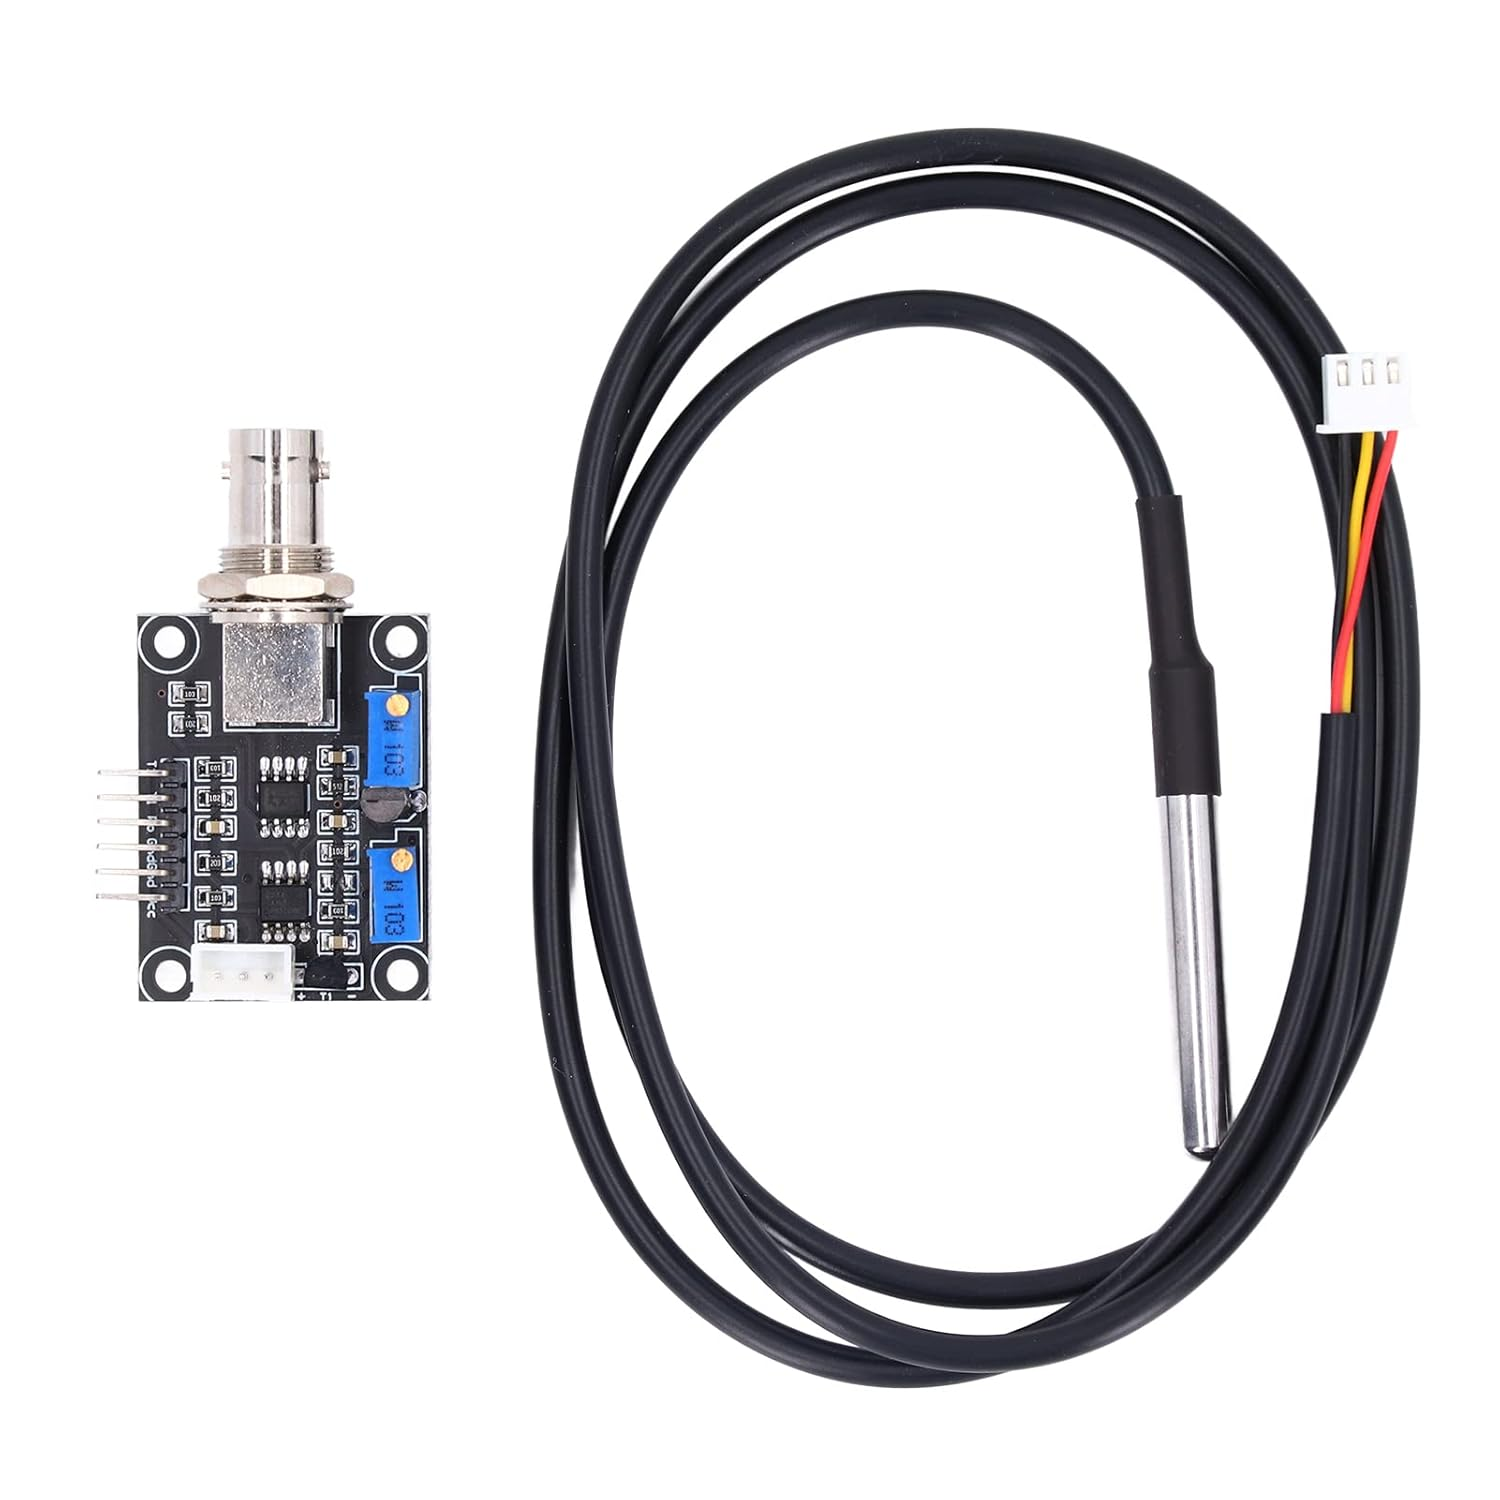
\includegraphics[width=0.49\linewidth]{figures/PH-Interface+Temperature} 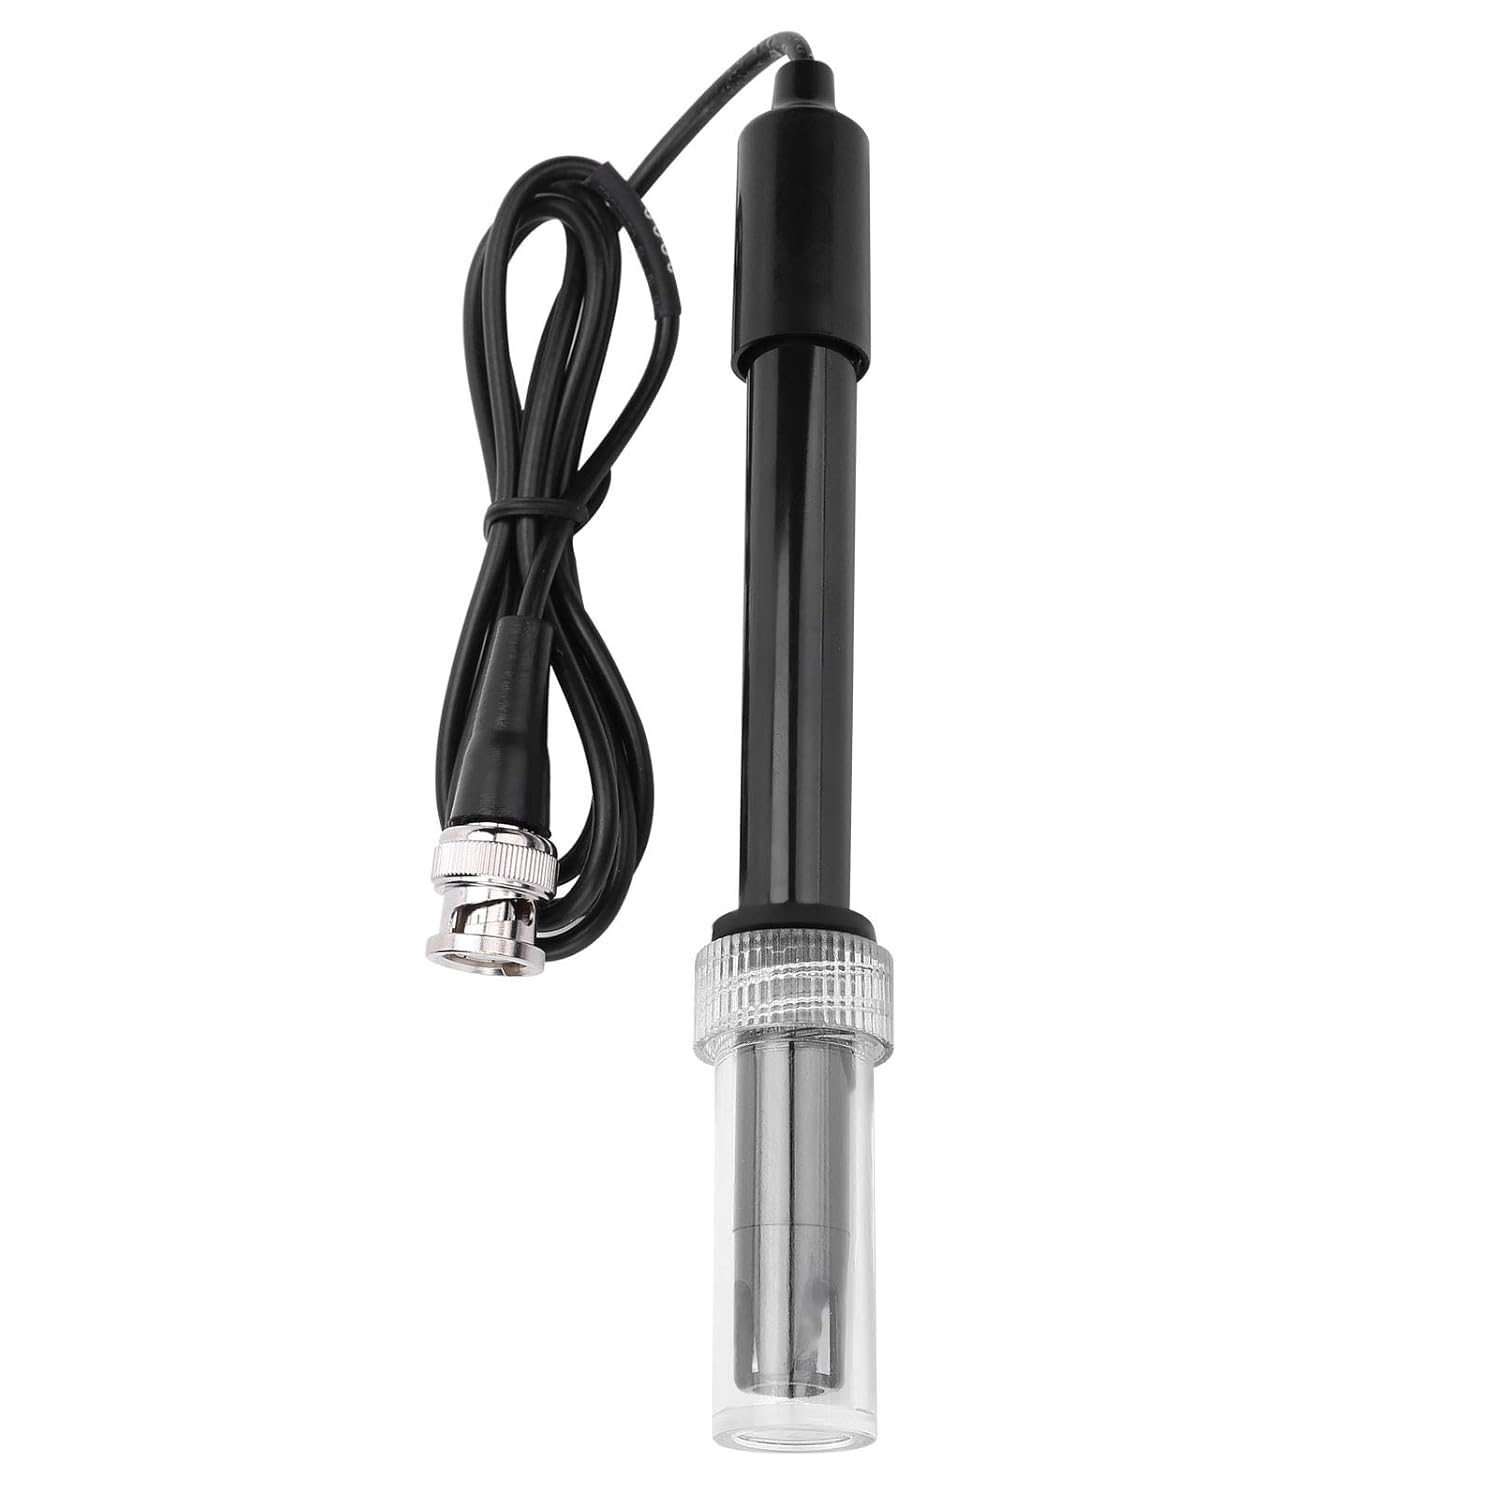
\includegraphics[width=0.49\linewidth]{figures/PH-Electrode}\\
    \scriptsize Typical pH-4502C style board + probe
  \end{column}
\end{columns}
\end{frame}

% \begin{frame}{pH + ESP32: Wiring \& Measurement Workflow}
% \begin{columns}[T,onlytextwidth]
%   \begin{column}{0.62\textwidth}
%     \begin{itemize}
% \item \textbf{Power:} many boards expect \textbf{5\,V} (check yours) + GND
% \item \textbf{Analog OUT $\rightarrow$ ESP32 ADC1}
% %             \begin{itemize}
% \item If OUT may exceed 3.3\,V: \textbf{divider} into ESP32
% \item Mittelung + stabile Abtastzeit verwenden (Elektroden reagieren langsam)
% %             \end{itemize}
% \item \textbf{Calibration:}
% %             \begin{itemize}
% \item measure buffers, adjust offset/slope (often 2 trim pots)
% \item store calibration constants in flash/NVS
% %             \end{itemize}
% \item Optional: Temperatursensor für \textbf{Temperaturkompensation}
%     \end{itemize}
%   \end{column}
%   \begin{column}{0.38\textwidth}
%     \centering
% %    \includegraphics[width=\linewidth]{figures/ph_board_closeup.jpg}\\
%     \scriptsize BNC + analog output to ADC
%   \end{column}
% \end{columns}
% \end{frame}

% ============================================================
% Device 4: GT-U7 GPS module (ASIN B0CNGWV7MN)
% ============================================================
\section[nosectionpage]{Global Positioning System (GPS)}
\begin{frame}{GT-U7 GPS Module (B0CNGWV7MN): What it Gives You}
\begin{columns}[T,onlytextwidth]
  \begin{column}{0.62\textwidth}
    \begin{itemize}
\item Liefert \textbf{Position + Zeit} von GNSS‑Satelliten
\item Outputs standard \textbf{NMEA sentences} over \textbf{UART serial}
\item Die Standard-Baudrate ist häufig \textbf{9600 bps}
\item Benötigt eine gute Antennenplatzierung (nahe Fenster / im Freien für den schnellsten Fix)
\item Typische Ausgänge:
            latitude, longitude, altitude, speed, UTC time, satellites in view
    \end{itemize}
  \end{column}
  \begin{column}{0.38\textwidth}
    \centering
    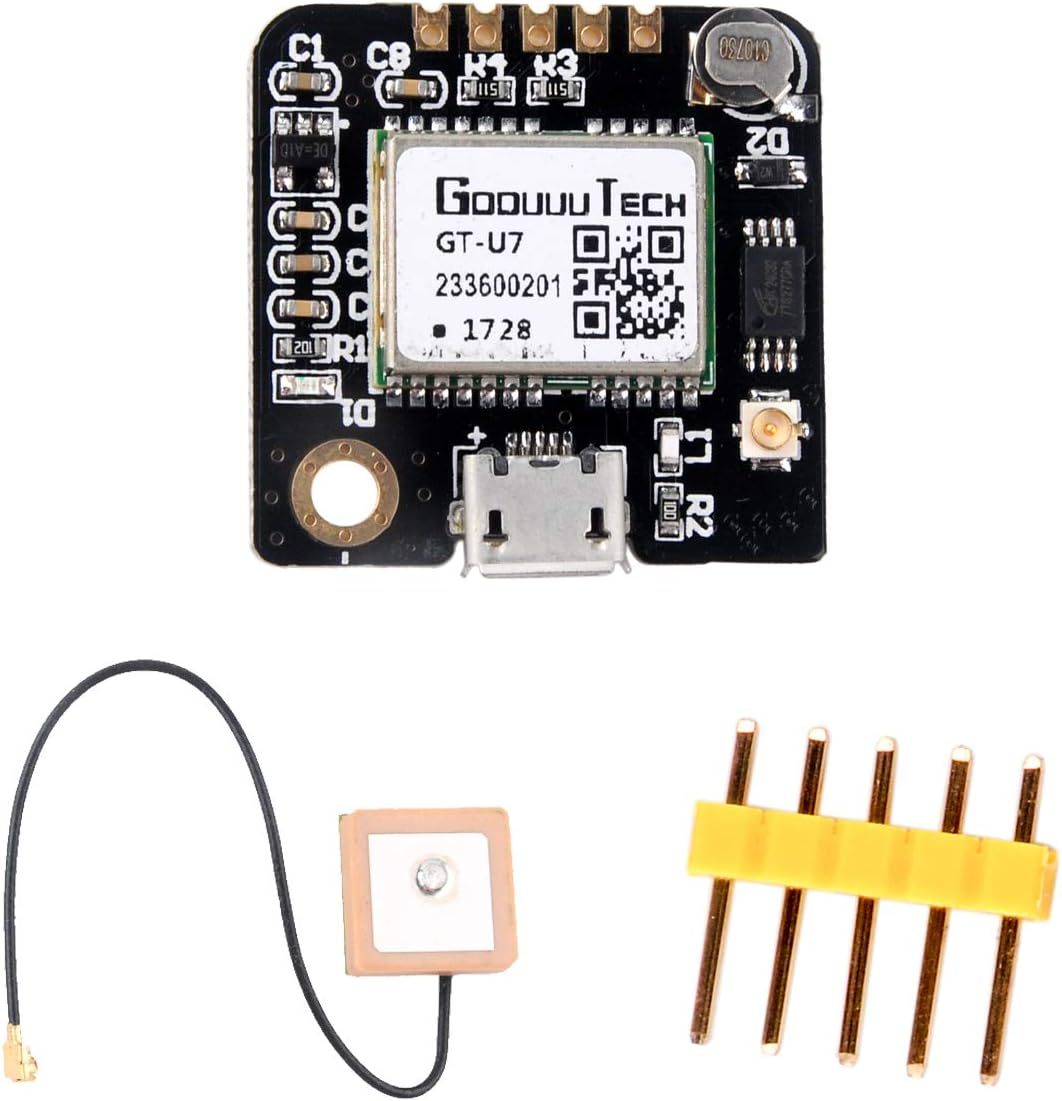
\includegraphics[width=0.7\linewidth]{figures/GPS-GT-U7}\\
    \scriptsize GT-U7 module (patch antenna + UART pins)
  \end{column}
\end{columns}
\end{frame}

% \begin{frame}{GT-U7 + ESP32: Wiring \& Decoding}
% \begin{columns}[T,onlytextwidth]
%   \begin{column}{0.62\textwidth}
%     \begin{itemize}
% \item \textbf{Power:} module supply (often 3.3--5\,V) + GND
% \item \textbf{UART wiring:}
% %             \begin{itemize}
% \item GPS \textbf{TX} $\rightarrow$ ESP32 \textbf{RX} (e.g., UART2)
% \item GPS \textbf{RX} $\leftarrow$ ESP32 \textbf{TX} (optional)
% \item Logikpegel prüfen; Pegelwandlung einsetzen, wenn TX des Moduls 5\,V ist
% %             \end{itemize}
% \item \textbf{Software:} NMEA mit TinyGPSPlus (Arduino) oder dem ESP‑IDF‑Parser auswerten
% \item Use-Case-Idee: GPS-Position zu MQTT-Telemetrie hinzufügen (Asset-Tracking / Bojen)
%     \end{itemize}
%   \end{column}
%   \begin{column}{0.38\textwidth}
%     \centering
% %    \includegraphics[width=\linewidth]{figures/gtu7_pins.jpg}\\
%     \scriptsize Pin labels help a lot in class
%   \end{column}
% \end{columns}
% \end{frame}

% ------------------------------------------------------------

\section[nosectionpage]{LoRa Interface}
\begin{frame}{LoRa SX1262: Was es ist}
\begin{columns}[T,onlytextwidth]
  \begin{column}{0.62\textwidth}
    \begin{itemize}
\item \textbf{SX1262 = sub-GHz LoRa transceiver} (radio chip, not a MCU)
\item Unterstützt \textbf{LoRa-Modulation} für große Reichweite + \textbf{(G)FSK} für Legacy-Modi
\item Kernmerkmal: \textbf{bis zu +22\,dBm Sendeleistung} (SX1261 typischerweise +15\,dBm)
\item Optimiert für \textbf{Low-Power}‑LPWAN‑Anwendungen
\item Typische Frequenzbänder: \textbf{EU868}, \textbf{US915}, weitere (abhängig von Modul + Antenne)
\item Used in: sensors, trackers, buoys, remote meters, industrial telemetry
    \end{itemize}
    \vspace{0.3em}
    \footnotesize
    Mental model: ESP32 does the application + protocol; SX1262 does the RF link.
  \end{column}

  \begin{column}{0.38\textwidth}
    \centering
    % Put a photo of a SX1262 module here (e.g., Waveshare Core1262-868M).
    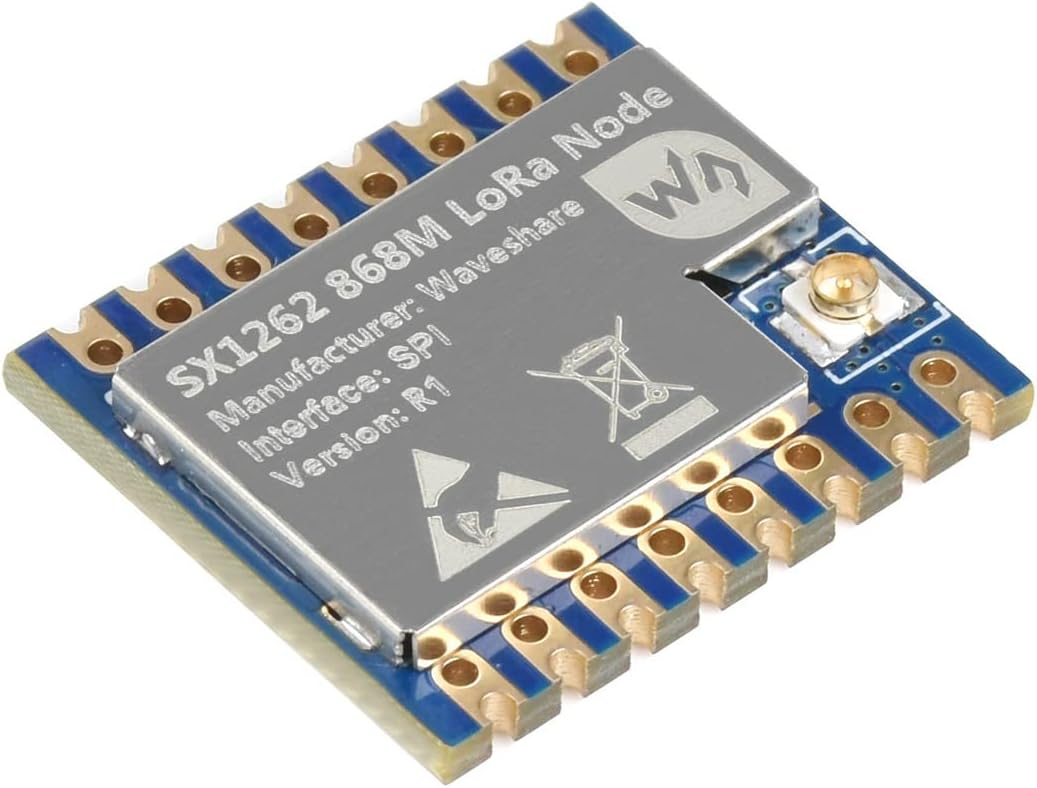
\includegraphics[width=0.8\linewidth]{figures/SX1262}\\
    \scriptsize SX1262 module (example)
  \end{column}
\end{columns}
\end{frame}

% ------------------------------------------------------------
\begin{frame}{SX1262 + ESP32: Wiring \& Software Pattern}
\begin{columns}[T,onlytextwidth]
  \begin{column}{0.55\textwidth}
    \begin{itemize}
\item Schnittstelle: \textbf{SPI} + einige Control-/Status-Pins:
        \begin{itemize}
\item \textbf{NSS/CS}, \textbf{SCK}, \textbf{MOSI}, \textbf{MISO}
\item \textbf{DIO1} (IRQ line, signals TX done / RX done / timeouts)
\item \textbf{BUSY} (Chip ist beschäftigt; Host muss vor dem SPI-Befehl warten)
\item \textbf{NRST} (reset)
         \end{itemize}
\item Antenne: auf \textbf{50\,($\Omega$)} auslegen und das richtige Band verwenden (EU868‑Antenne für EU868)
\item Software options:
         \begin{itemize}
\item \textbf{Radio-only} (P2P LoRa): RadioLib, SX126x driver
\item \textbf{LoRaWAN} (TTN): LoRaWAN stack + SX1262 radio driver
        \end{itemize}
\item Typisches RadioLib-Konstruktor-Pattern: \texttt{Module(NSS, DIO1, RST, BUSY)}
    \end{itemize}
  \end{column}

  \begin{column}{0.45\textwidth}
    \centering
    % Put a pinout/connection diagram here (e.g., Waveshare wiki pinout).
    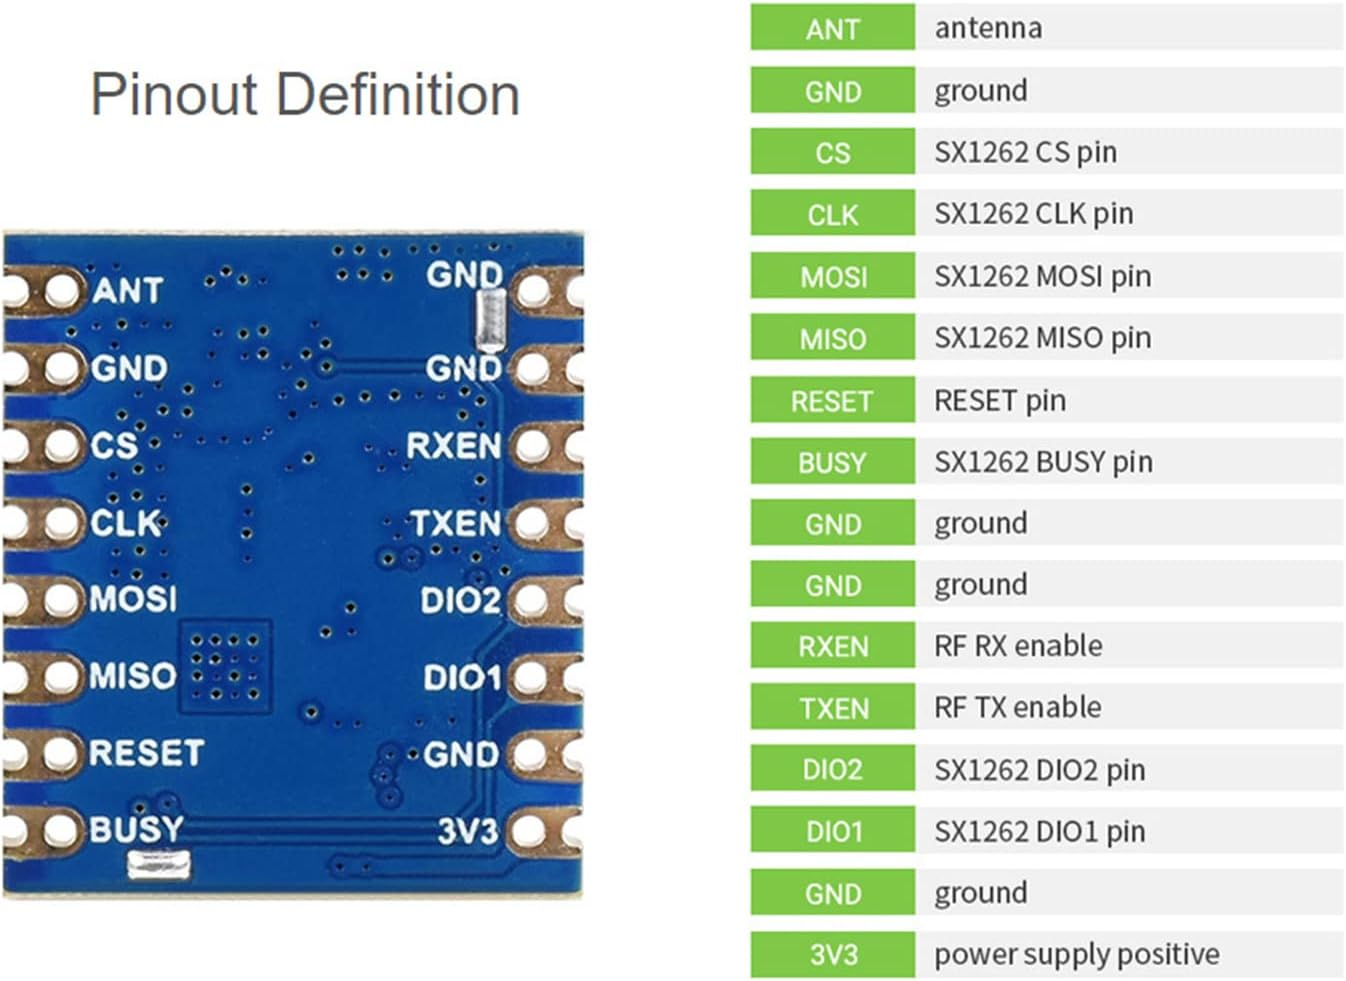
\includegraphics[width=0.9\linewidth]{figures/SX1262-pinout}\\
    \scriptsize Pinout / wiring overview (example)
  \end{column}
\end{columns}
\end{frame}

\section[withsectionpage]{Wiring Everything together}
\begin{frame}[plain]
\makebox[\linewidth]{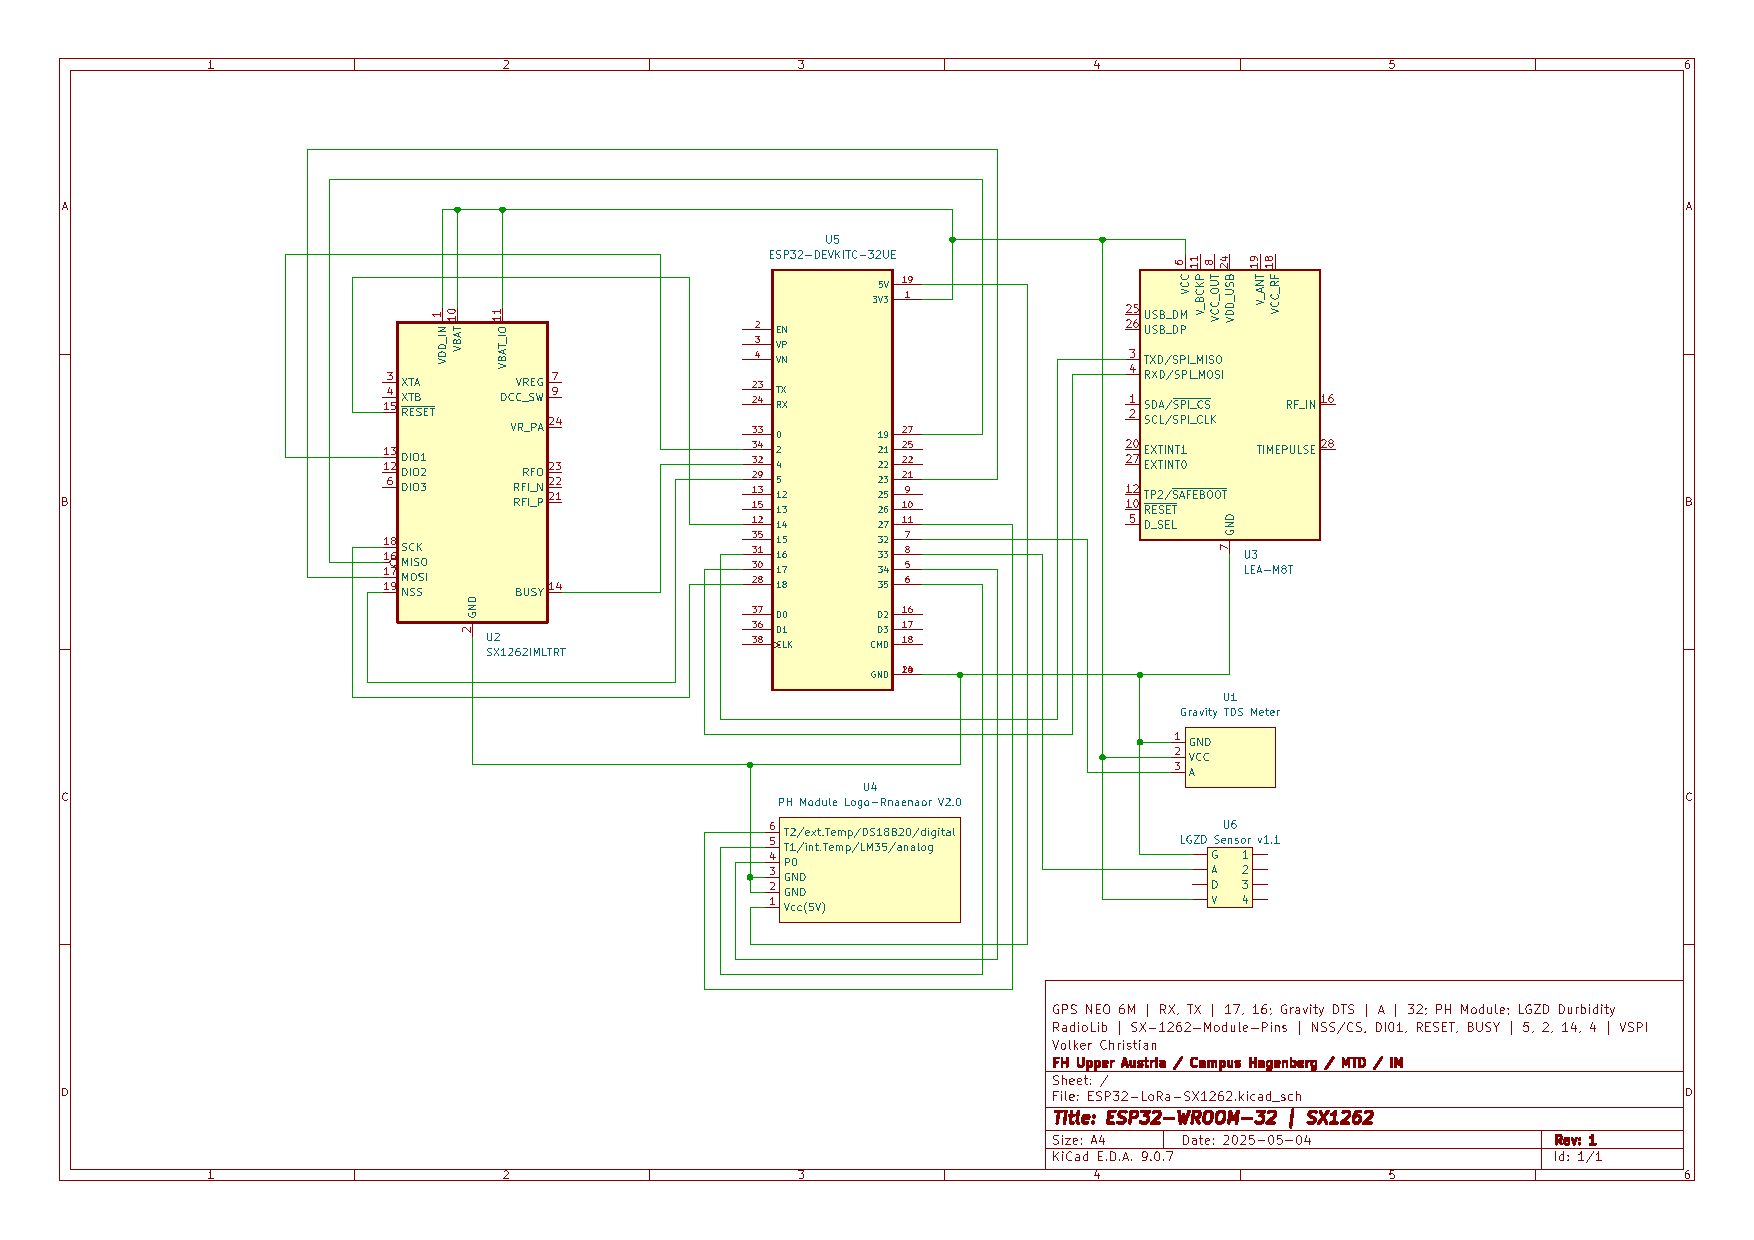
\includegraphics[width=\paperwidth,height=\paperheight,keepaspectratio]{figures/ESP32-SX1262-PH-Temp-TDS-Turbidity}}
\end{frame}
